\begin{frame}{$d(K^-, n)"\pi^{\pm}\Sigma^{\mp}"$ event selection}
  \begin{tabular}{cc}
    \begin{minipage}{0.5\hsize}
      { \scriptsize
        $d(K^-, n \pi^+ \pi^-)"n"$ was selected by 2$\sigma$.\\
        $K^- d \rightarrow K^0 n n $ was selected by 3$\sigma$.\\
        $K^- d \rightarrow \Sigma^{\pm}\pi^{\mp} n_{miss}$ was rejected by 3$\sigma$.
      }
      \begin{figure}
        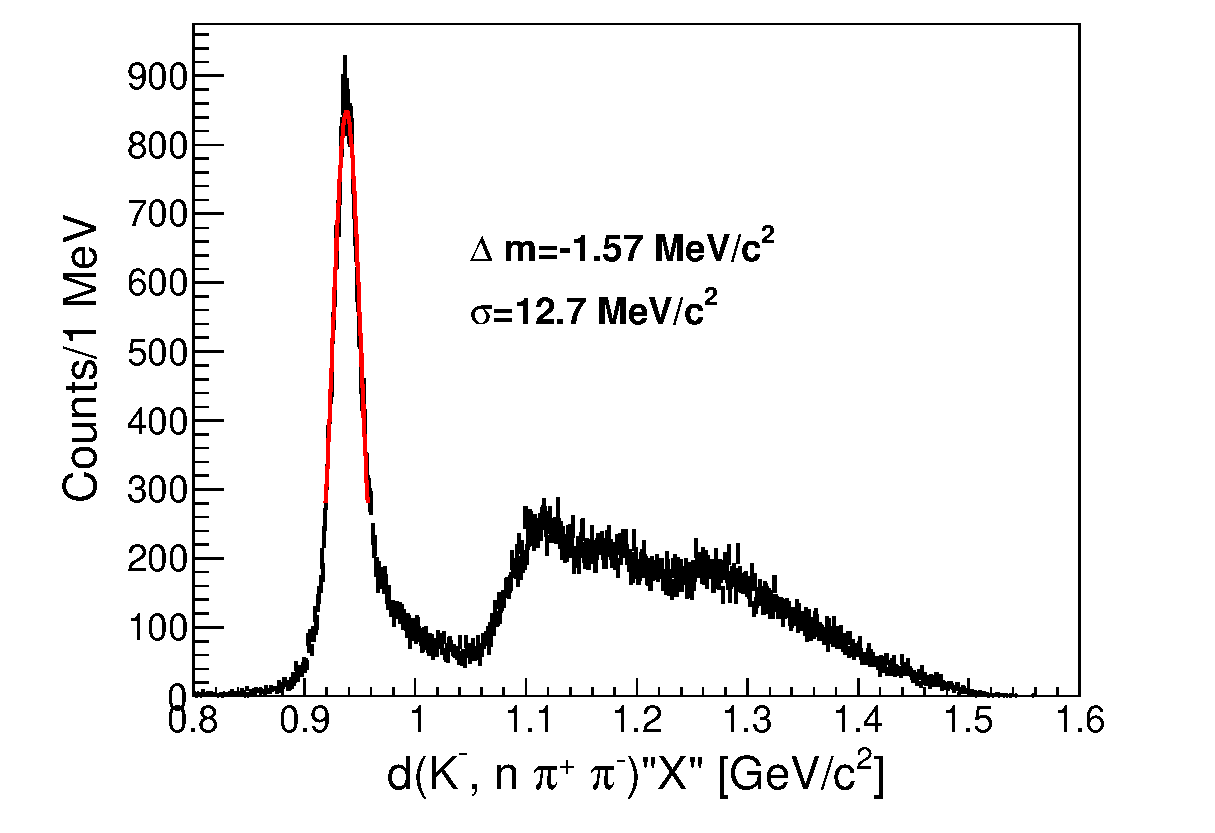
\includegraphics[width=5cm]{../pic/Run78/KN_ana_NC170_2sigma/KNpipi_MM_woFit.eps}
      \end{figure}
    \end{minipage}

    \begin{minipage}{0.5\hsize}
      \begin{figure}
        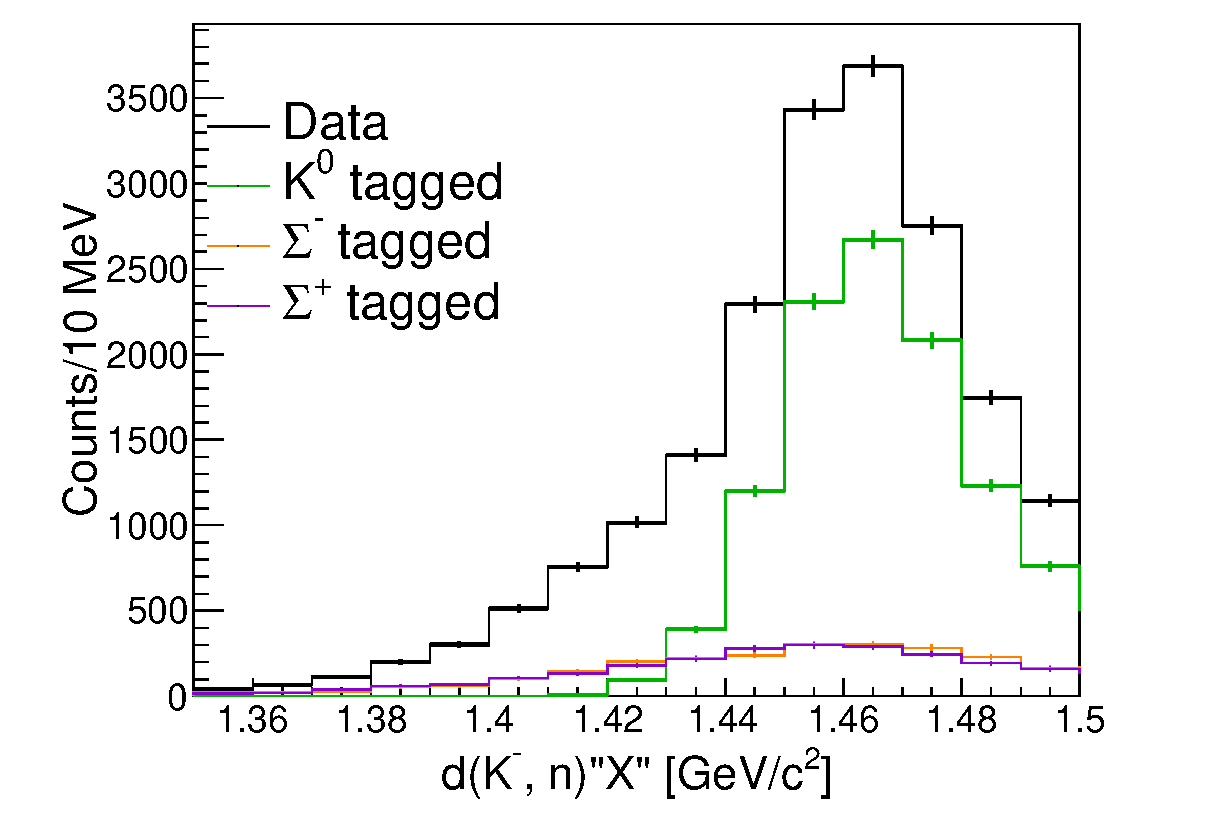
\includegraphics[width=6cm]{../pic/Run78/KN_ana_NC170_2sigma/KN_MM_all.eps}
      \end{figure}
    \end{minipage}
  \end{tabular}

  \begin{tabular}{cc}
    \begin{minipage}{0.33\hsize}
      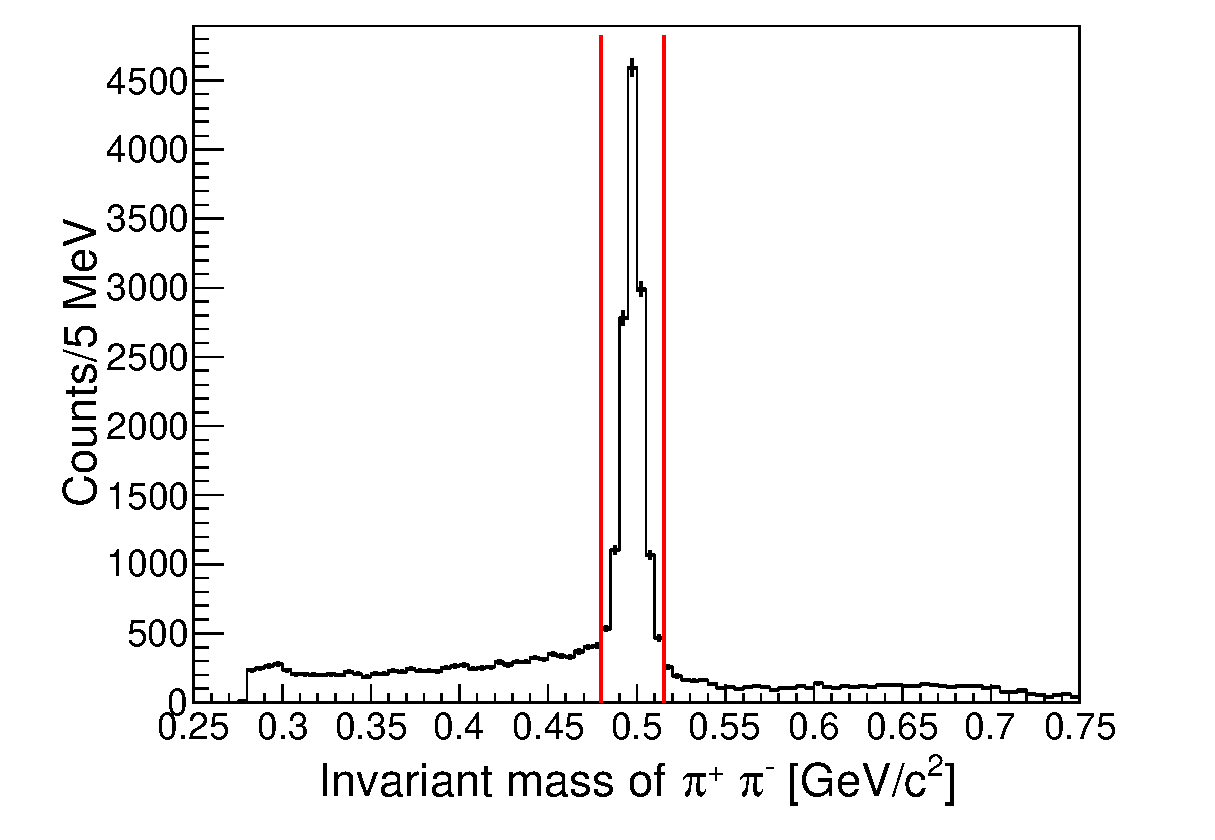
\includegraphics[width=3cm]{../pic/Run78/KN_ana_NC170_2sigma/IM_pipi_woFit.eps}
    \end{minipage}

    \begin{minipage}{0.33\hsize}
      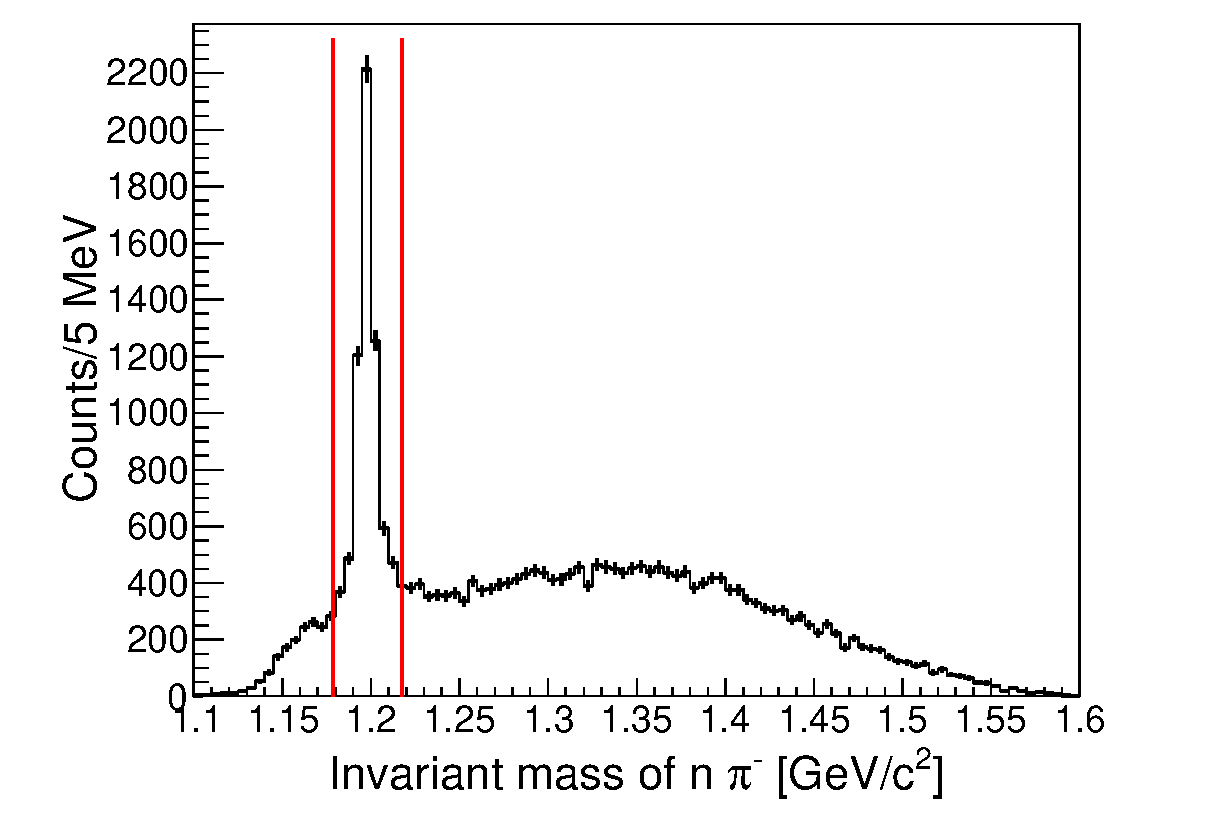
\includegraphics[width=3cm]{../pic/Run78/KN_ana_NC170_2sigma/IM_npim_woFit.eps}
    \end{minipage}

    \begin{minipage}{0.33\hsize}
      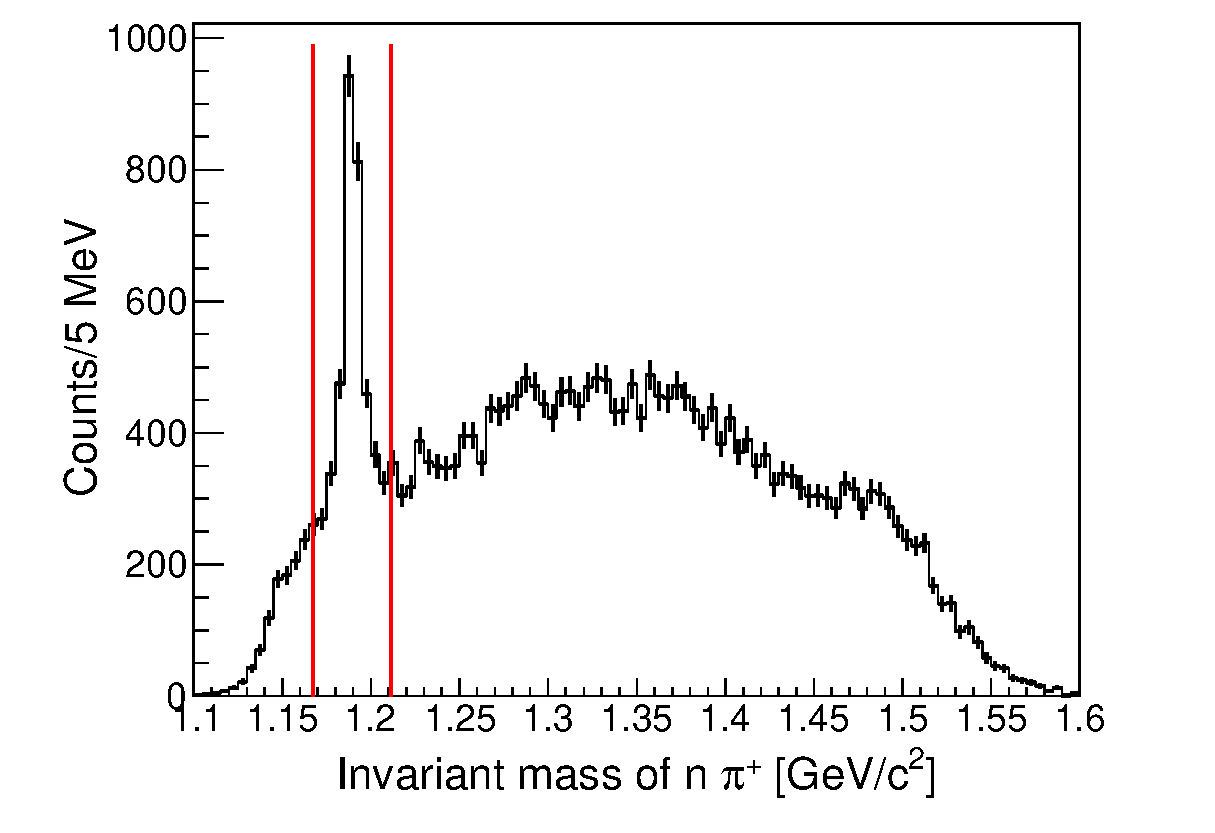
\includegraphics[width=3cm]{../pic/Run78/KN_ana_NC170_2sigma/IM_npip_woFit.eps}
    \end{minipage}
  \end{tabular}
\end{frame}
